\section{Aufbau}
\label{sec:Aufbau}


Für den Versuch wird ein Aufbau wie in Abbildung \ref{fig:Aufbau} benutzt.
An das Zählrohr ist die Spannung $U$ angeschlossen.
Der Ladungsimpuls fließt über den Widerstand $R$ ab und erzeugt dort einen Spannungsimpuls.
Dieser wird über den Kondensator C ausgekoppelt, im Verstärker vergrößert und im Zählgerät registriert.
Außderdem kann der Spannungsimpuls über ein Oszillographen betrachtet werden.
\begin{figure}
  \centering
  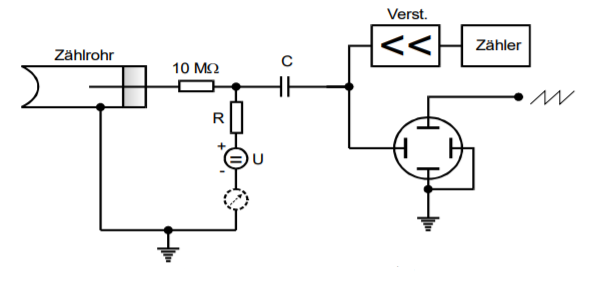
\includegraphics[height=6cm]{data/Aufbau.png}
  \caption{Skizze des Versuchaufbaus. \cite{V703}}
  \label{fig:Aufbau}
\end{figure}
